\chapter{Problem Statement}
\label{sec:problem-statement}

In this chapter we expound the fundamentals of what we'll be working on in later chapters. We begin by defining the structure of the datasets---\emph{event sequences} composed of \emph{events}, each of a certain type and occurring at a certain time.

Next, we define patterns, named \emph{episodes} in sequence pattern mining, and cover the classes of episodes we will be mining. We define several \emph{frequency measures} proposed by different researchers, which quantify how interesting an episode is, so that we can find the most interesting episodes in a sequence.

Finally, from episodes we can construct \emph{association rules}, which can uncover correlations between the different events in an event sequence. On association rules, \emph{confidence measures} are defined, where high-scoring rules denote high correlation between events.

\section{Event sequences}

\begin{definition}
A \emph{sequence event}, or \emph{event} for short, is a pair $ (A, t) $ where $ A \in \Sigma $ is an event type from a given set of event types $ \Sigma $, and $ t $ is an integer timestamp, denoting the point in time at which the event occurred.
\end{definition}

\begin{definition}
An \emph{event sequence} $ \boldsymbol{s} $ is a triple $ (s, T_s, T_e) $, where $ s $ is an ordered sequence of events
\begin{align*}
s = \langle (A_1, t_1), (A_2, t_2), \, \ldots, \, (A_n, t_n) \rangle
\end{align*}
such that $ t_i \leq t_{i + 1} $ for all $ i = 1, \, \ldots, \, n - 1 $, and any given pair $ (A, t) $ appears at most once.

With $ \boldsymbol{s}_i $ we refer to the pair $ (A_i, t_i) $ in $ s $.

$ T_s $ and $ T_e $ are timestamps such that $ T_s \leq t_1 $ and $ t_n < T_e $. They mark the beginning and the end of the sequence, respectively.

If a sequence event $ (A, t) $ is in $ s $, we say that the event \emph{occurs} in $ \boldsymbol{s} $ at timestamp $ t $.
\end{definition}

Figure~\ref{fig:event-sequence} shows a visualization of a possible event sequence.

\newcommand{\sequencetickmarks}[3]
{
% args: (number of tick marks, x of first tick mark, y of first tick mark)
    \pgfmathsetmacro\secondtickmark{#2+0.5}
    \pgfmathsetmacro\lasttickmark{#2+0.5*#1}

    \draw (#2,#3) -- (\lasttickmark,#3);

    \foreach \x in {#2,\secondtickmark,...,\lasttickmark}
        \draw (\x,#3) -- +(0,3pt);
}

\newcommand{\sequenceeventtypes}[4]
{
% args: (x of first event, y, t of first event, list of t/A pairs)
    \pgfmathsetlengthmacro\nodeheight{(#2)+(.8em)}

    \foreach \t/\eventtype [evaluate=\t as \x using (\t-#3)*0.5+(#1)] in {#4}
    {
        \node [font=\vphantom{$ fbd $}] at (\x,#2) {$ \eventtype $};
        \node (t\t) [inner sep=0] at (\x,\nodeheight) {};
    }
}

\newcommand{\windowthingy}[2]
{
% args: starting position (leftmost point of horizontal line), number of timestamps
    \pgfmathsetmacro\windowthingylength{#2*0.5-0.1}
    \draw [thick] #1 ++(0,3pt) -- ++(0,-3pt) -- ++(\windowthingylength,0) -- ++(0,3pt);
}

\newcommand{\examplesequence}
{
    \sequencetickmarks{23}{-5.5}{0}

    \sequenceeventtypes{-5.5}{1em}{30}{32/c,33/f,34/b,35/b,38/c,40/d,41/a,44/b,46/e,47/a,48/e,49/c};
}

\newcommand{\examplesequencetimestamps}
{
    \foreach \x [evaluate=\x as \timestamp using int((\x*2)+41)] in {-5.5,-3,...,5.5}
    \node at (\x,-1em) {$ \timestamp $};
}

\begin{figure}[h]
\centering

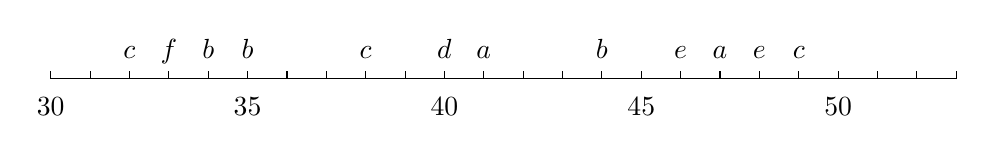
\begin{tikzpicture}

\examplesequence
\examplesequencetimestamps

\end{tikzpicture}

\caption{A visual representation of a sequence.}
\label{fig:event-sequence}
\end{figure}

Note that multiple events can occur at the same timestamp, if they have different event types. Some implementations do not allow this, however.

For the sake of simplicity, we use the notation $ s_1 \cdots s_n $ to mean the sequence $ (\langle (s_1, 1), \ldots,\allowbreak(s_n, n) \rangle, 1, n + 1) $.

Since sequences are allowed to be very long, and we are mostly looking for events occurring relatively close to each other, we would like to be able to consider parts of a sequence while ignoring the rest of it. Therefore we use the concept of a window on a sequence.

\begin{definition}
Given a sequence $ \boldsymbol{s} = (s, T_s, T_e) $ and two timestamps $ t_s $ and $ t_e $,
% such that $ t_s < T_e $ and $ T_s < t_e $
we define a \emph{window} on $ \boldsymbol{s} $ to be an event sequence $ \boldsymbol{s}[t_s, t_e) = (w, t_s, t_e) $ where $ w $ contains all events $ (A, t) $ in $ s $ where $ t_s \leq t < t_e $. We call $ \rho = t_s - t_e $ the \emph{width} of the window. $ \boldsymbol{s}[t_s, t_e) $ is a \emph{proper} subwindow of $ \boldsymbol{s} $ if $ w $ contains fewer events than $ \boldsymbol{s} $. Two windows $ \boldsymbol{s}[a, b) $ and $ \boldsymbol{s}[c, d) $ \emph{overlap} if $ [a, b) \cap [c, d) \neq \emptyset $. Otherwise we call them non-overlapping, or \emph{disjoint}.
\end{definition}

Note that in the previous definition, $ t_s $ and $ t_e $ do not have to be within the sequence itself. A window on a sequence can thus start before the sequence starts, or end after the sequence ends. This will be important for some of the algorithms.

Figure~\ref{fig:windows} illustrates a window on the sequence of figure~\ref{fig:event-sequence}.

\begin{figure}[h]
\centering

\begin{tikzpicture}

\examplesequence
\examplesequencetimestamps

\draw [very thick] (1.5,-0.6) -- ++(0,-3pt) -- ++(2.4,0) -- ++(0,3pt);

\draw [->,very thick] (2.75,-0.8) -- ++(0,-0.5);

\draw (1.5,-2) -- ++(2.4,0);

\foreach \x in {1.5,2,...,3.5}
    \draw (\x,-2) -- ++(0,3pt);

\foreach \x/\label in {
    1.5/b,
    2.5/e,
    3/a,
    3.5/e}
    \path (\x,-2) ++(0,1em) node [enoughdamnvspace] {$ \label $};

\path (1.5,-2) ++(0,-1em) node {$ 44 $};

\node [anchor=east] at (1,-2) {Contents of window $ \boldsymbol{s}[44,49) $:};

\end{tikzpicture}

\caption{A window of width 5 on a sequence $ \boldsymbol{s} $.}
\label{fig:windows}
\end{figure}

\section{Episodes}

Given a pattern and a sequence, we would like to quantify how interesting the pattern is. One way to define \emph{interesting} is how often it occurs in the sequence. While other interpretations of \emph{interestingness} exist [TODO cite (?)], we will mainly focus on \emph{frequency measures}, some of which we'll discuss in section~\ref{sec:interestingness-measures-episodes}. First we formally define patterns.

% TODO ^ cite Geoff Webb maybe? ^

\begin{definition}
An \emph{episode} $ \alpha $ is a directed acyclic graph with labelled nodes, that is, $ \alpha = (V, E, lab) $, where $ V = (v_1, \ldots, v_k) $ is the set of nodes, $ E $ is the set of directed edges, and \emph{lab} is a function $ lab \colon V \rightarrow \Sigma $, mapping each node $ v_i $ to an event type. If $ lab(v) = A $, then we say that node $ v $ is of (event) type $ A $, and that $ \alpha $ contains $ A $, or $ A $ is in $ \alpha $.
\end{definition}

We write $ | \alpha | $ to mean the number of nodes in an episode's graph. We call $ | \alpha | $ the \emph{size} of $ \alpha $.

\begin{definition}
A node $ n $ in an episode graph is a \emph{descendant} of a node $ m $ if there is a path from $ m $ to $ n $. Conversely $ m $ is an \emph{ancestor} of $ n $ in that case.
\end{definition}

\begin{definition}
Given a sequence $ \boldsymbol{s} $ and an episode $ \alpha $ we say that $ \boldsymbol{s} $ \emph{covers} $ \alpha $, or $ \alpha $ \emph{occurs in} $ \boldsymbol{s} $, if there is an injective map $ f $ mapping each node $ v_i $ to a valid index such that:
\begin{enumerate}
\item the node $ v_i $ in $ \alpha $ and the corresponding sequence element $ \boldsymbol{s}_{f(v_i)} $ are of the same event type: $ \boldsymbol{s}_{f(v_i)} = lab(v_i) $, and
\item if there is an edge $ (v_i, v_j) $ in $ \alpha $, then we must have $ f(v_i) < f(v_j) $. In other words, the ancestors of $ v_j $ must occur in $ \boldsymbol{s} $ before $ v_j $. If the mapping $ f $ is surjective, that is, all events in $ \boldsymbol{s} $ are used, we will say that $ \boldsymbol{s} $ is an \emph{instance} of $ \alpha $.
\end{enumerate}
\end{definition}

More intuitively, the above definition says that an episode occurs in a sequence if the event types corresponding to the episode's nodes appear in the sequence, respecting the order of the episode's edges.

\begin{definition}
Episodes $ \alpha $ and $ \beta $ are said to be \emph{equivalent} if each sequence that covers $ \alpha $ also covers $ \beta $, and vice versa.
\end{definition}

In this thesis, we'll be limiting ourselves to two subcategories of episodes:
\begin{itemize}
\item \textbf{Parallel episodes.} A parallel episode is an episode for which the set of edges is empty. As such, no constraints are placed on the order in which event types occur in a sequence. An example is shown in figure~\ref{fig:episode-graphs-parallel}, and figure~\ref{fig:occurrences} (right) shows an occurrence in a sequence. In text we'll write parallel episodes by their event types using the following notation:
\begin{align*}
    \{ A_1, A_2, \ldots, A_n \}
\end{align*}
by which we mean a parallel episode with $ n $ nodes, and event types $ A_1 $ through $ A_n $. Note that though the notation reminds strongly of the notation for a mathematical set, it does not actually represent a set: a parallel episode $ \{ a, a, b, c \} $ is not equivalent to an episode $ \{ a, b, c \} $.

\item \textbf{Serial episodes.} A serial episode is an episode for which the edges cause the nodes to have a total order. That way, in any occurrence of a serial episode in a sequence, the event types appear in the same order. Figure~\ref{fig:episode-graphs-serial} shows an example, and figure~\ref{fig:occurrences} (left) shows an occurrence in a sequence.

% Sometimes it is useful to describe serial episodes in their strict form, in which there is a direct edge between any two nodes. Figure~\ref{fig:episode-graphs-serial-strict} shows a strict episode which is equivalent to the episode in figure~\ref{fig:episode-graphs-serial}.

While serial episodes have a different graph in this form, their meaning is the same, since they enforce the same order on the occurrence of events in the sequence to satisfy an occurrence of a serial episode.

For serial episodes we will use the notation
\begin{align*}
    A_1 \to A_2 \to \cdots \to A_n
\end{align*}
where $ A_i $ is the event type of the $ i $-th node, and a node of event type $ A_i $ is an ancestor of a node of event type $ A_j $ if $ i < j $.

\end{itemize}

\begin{figure}

\begin{subfigure}[b]{\textwidth}
\centering
\begin{tikzpicture}

\node (n 1) [circly,label={$ c $},enoughdamnvspace] at (-3,-3pt) {$ v_1 $};
\node (n 2) [circly,label={$ a $},enoughdamnvspace] at (-1, 3pt) {$ v_2 $};
\node (n 3) [circly,label={$ b $},enoughdamnvspace] at ( 1,-3pt) {$ v_3 $};
\node (n 4) [circly,label={$ b $},enoughdamnvspace] at ( 3, 3pt) {$ v_4 $};

\end{tikzpicture}
\caption{parallel}
\label{fig:episode-graphs-parallel}
\end{subfigure}

\par\bigskip

\begin{subfigure}[b]{\textwidth}
\centering
\begin{tikzpicture}

\node (n 1) [circly,label={$ b $},enoughdamnvspace] at (-3,0) {$ v_1 $};
\node (n 2) [circly,label={$ a $},enoughdamnvspace] at (-1,0) {$ v_2 $};
\node (n 3) [circly,label={$ c $},enoughdamnvspace] at ( 1,0) {$ v_3 $};
\node (n 4) [circly,label={$ d $},enoughdamnvspace] at ( 3,0) {$ v_4 $};

\draw [->] (n 1) -- (n 2);
\draw [->] (n 2) -- (n 3);
\draw [->] (n 3) -- (n 4);

\end{tikzpicture}
\caption{serial}
\label{fig:episode-graphs-serial}
\end{subfigure}

\par\bigskip

\iffalse
\begin{subfigure}[b]{\textwidth}
\centering
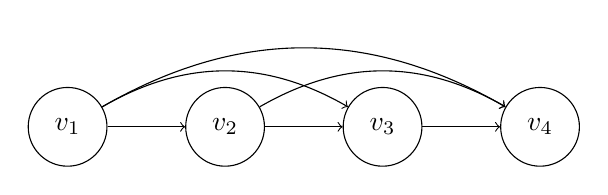
\begin{tikzpicture}

\node (n 1) [circly] at (-3,0) {$ v_1 $};
\node (n 2) [circly] at (-1,0) {$ v_2 $};
\node (n 3) [circly] at ( 1,0) {$ v_3 $};
\node (n 4) [circly] at ( 3,0) {$ v_4 $};

\draw [->] (n 1) -- (n 2);
\draw [->] (n 2) -- (n 3);
\draw [->] (n 3) -- (n 4);

\draw [->] (n 1) to [bend left=30] (n 3);
\draw [->] (n 2) to [bend left=30] (n 4);
\draw [->] (n 1) to [bend left=30] (n 4);

\end{tikzpicture}

\caption{serial, strict}
\label{fig:episode-graphs-serial-strict}
\end{subfigure}
\fi

\caption{An example of an episode graph for each of the episode class we will consider, with the event types shown above the nodes.}

\label{fig:episode-graphs}
\end{figure}

\begin{figure}
\centering

\begin{tikzpicture}

\examplesequence
\examplesequencetimestamps

% serial episode

\node (serC) at (-5,2.5) [smallnode,label={$ c $}] {};
\node (serF) at (-4,2.5) [smallnode,label={$ f $}] {};
\node (serB) at (-3,2.5) [smallnode,label={$ b $}] {};

\draw [->,very thick] (serC) -- (serF);
\draw [->,very thick] (serF) -- (serB);

\draw [->] ([yshift=-3pt]serC.south) .. controls +(0,-1) and +(0,1) .. (t32);
\draw [->] ([yshift=-3pt]serF.south) .. controls +(0,-1) and +(0,1) .. (t33);
\draw [->] ([yshift=-3pt]serB.south) .. controls +(0,-1) and +(0,1) .. (t34);

% parallel episode

\node (parB) at (3,2.6) [smallnode,label={$ b $}] {};
\node (parE1) at (2,1.8) [smallnode,label={$ e $}] {};
\node (parE2) at (4.5,2.4) [smallnode,label={$ e $}] {};
\node (parC) at (3.5,2) [smallnode,label={$ c $}] {};

\draw [->] ([yshift=-3pt]parB.south) .. controls +(0,-1) and +(0,1) .. (t44);
\draw [->] ([yshift=-3pt]parE1.south) .. controls +(0,-0.5) and +(0,0.5) .. (t46);
\draw [->] ([yshift=-3pt]parE2.south) .. controls +(0,-1) and +(0,1) .. (t48);
\draw [->] ([yshift=-3pt]parC.south) .. controls +(0,-0.5) and +(0,0.5) .. (t49);

\end{tikzpicture}

\caption{Showing an occurrence of a serial episode $ c \to f \to b $ and an occurrence of a parallel episode $ \{ b, c, e, e \} $ in the sequence of figure~\ref{fig:event-sequence}.}
\label{fig:occurrences}
\end{figure}

Because we only consider parallel and serial episodes, it is easy to represent an episode in a data structure---we don't need to explicitly store a graph with nodes and edges:
\begin{itemize}
\item Parallel episodes can be stored in an array, where each element is simply the event type of the episode. Strictly speaking, the order of the elements in the array doesn't matter, but it can be useful for them to follow some order on the set of event types. In that way each parallel episode has a unique array representation. Figure~\ref{fig:parallel-representation} shows the representation visually.

\tikzset{circly/.style={draw,circle,minimum size=1cm},
    arraycell/.style={draw,rectangle,minimum size=1cm,node distance=0}}

\begin{figure}[h]
\centering

\begin{tikzpicture}

\node (n 1) [circly,label=above:$ c $] at (-3,-3pt) {$ v_1 $};
\node (n 2) [circly,label=above:$ a $] at (-1, 3pt) {$ v_2 $};
\node (n 3) [circly,label=above:$ b $] at ( 1,-3pt) {$ v_3 $};
\node (n 4) [circly,label=above:$ a $] at ( 3, 3pt) {$ v_4 $};

\node [left=of n 1] {episode graph};

\draw [->] (0,-1) -- node [left=0.5cm] {sort the event types into an array} +(0,-1.5);

\node (a 1) [arraycell,enoughdamnvspace] at (-2,-3.5) {$ a $};
\node (a 2) [arraycell,right=of a 1,enoughdamnvspace] {$ a $};
\node (a 3) [arraycell,right=of a 2,enoughdamnvspace] {$ b $};
\node (a 4) [arraycell,right=of a 3,enoughdamnvspace] {$ c $};

\end{tikzpicture}

\caption{A parallel episode's graph representation, with the label of each node shown above, and its array representation.}

\label{fig:parallel-representation}
\end{figure}

\item Serial episodes can also be stored in an array, but here the order of the elements is defined by the edges of the episode. That is, the event types are ordered according to a topological sort of the nodes. Figure~\ref{fig:serial-representation} shows this visually.
\end{itemize}

\begin{figure}[h]
\centering

\begin{tikzpicture}

\node (n 1) [circly,label=above:$ a $] at (-3,0) {$ v_1 $};
\node (n 2) [circly,label=above:$ c $] at (-1,0) {$ v_2 $}
    edge [pre] (n 1);
\node (n 3) [circly,label=above:$ b $] at (1, 0) {$ v_3 $}
    edge [pre] (n 2);
\node (n 4) [circly,label=above:$ a $] at (3, 0) {$ v_4 $}
    edge [pre] (n 3);

\node [left=of n 1] {episode graph};

\draw [->] (0,-1) -- node [left=0.5cm,align=right] {store event types into array,\\preserving toplogical ordering} +(0,-1.5);

\node (a 1) [arraycell,enoughdamnvspace] at (-2, -3.5) {$ a $};
\node (a 2) [arraycell,right=of a 1,enoughdamnvspace] {$ c $};
\node (a 3) [arraycell,right=of a 2,enoughdamnvspace] {$ b $};
\node (a 4) [arraycell,right=of a 3,enoughdamnvspace] {$ a $};

\end{tikzpicture}

\caption{A serial episode's graph representation, with the label of each node shown above, and its array representation.}
\label{fig:serial-representation}
\end{figure}

When discussing the algorithms we will mostly consider their array representation, and address the $ i $-th element of an episode array $ \alpha $ with $ \alpha [i] $.

\begin{definition}
Given two episodes $ \alpha $ and $ \beta $, we say that $ \alpha $ is a \emph{subepisode} of $ \beta $, denoted $ \alpha \subseteq \beta $, if the set of all sequences that cover $ \beta $ is a subset of the set of all sequences that cover $ \alpha $. $ \alpha $ is a \emph{proper subepisode} of $ \beta $, denoted $ \alpha \subset \beta $, if $ \alpha \subseteq \beta $ and $ \alpha $ and $ \beta $ are not equivalent.
\end{definition}

Of course, considering all event sequences that cover an episode is an impossible task, so the above definition does not give rise to a practical way of determining whether one episode is a subepisode of another. Instead we must look at the episodes themselves, and reason about all of the ways in which they might occur in a sequence. For parallel and serial episodes, it is quite straightforward to do so, as described below. More general cases have been reasoned about~\cite{tatti2012mining}, but are beyond the scope of this thesis.

\begin{itemize}
\item A parallel episode $ \alpha $ is a subepisode of a parallel episode $ \beta $ if:
\begin{enumerate}
\item $ | V(\alpha) | \leq | V(\beta) | $, and
\item for each event type $ A $ in $ \alpha $, the number of nodes $ v $ in $ \alpha $ for which $ lab(v) = A $, is no greater than the number of nodes for which the same holds in $ \beta $.
\end{enumerate}
\item A serial episode $ \alpha $ is a subepisode of a serial episode $ \beta $ if:
\begin{enumerate}
\item the conditions for parallel episodes are satisfied, and additionally
\item if node $ v $ is an anchestor of node $ u $ in $ \alpha $, then there exist nodes $ u', v' $ in $ \beta $ such that $ u' $ is an anchestor of $ v' $ in $ \beta $ and $ lab(u) = lab(u') $ and $ lab(v) = lab(v') $. Put more simply, the ordering of event types must be preserved.
\end{enumerate}
\end{itemize}

\section{Frequency measures for episodes}
\label{sec:interestingness-measures-episodes}

Now that we have defined patterns on event sequences, we would like to be to be able to quantify how interesting a pattern is in regard to a sequence.

Traditionally, the most common interpretation of \emph{interestingness} is frequency, which expresses how often an episode occurs in the sequence. The more often an episode occurs, the more interesting it is considered to be.

Exactly how the frequency of an episode in a sequence should be defined, is not immediately clear. We will present three methods to measure the frequency of an episode. In a later section, we implement a mining algorithm based on them.

In data mining, the main challenge is how to mine information efficiently. In particular, exponential pattern growth is problematic. For itemset mining, the Apriori algorithm \cite{agrawal1994fast} was able to prune large amounts of itemsets because an itemset can only be frequent if all of its subsets are frequent. In sequential pattern mining, patterns explosion is even worse than in itemset mining. However, we can employ a similar technique if we define \emph{monotonically decreasing} measures.

\begin{definition}
A frequency measure is \emph{monotonically decreasing} if each episode is at least as frequent as any of its superepisodes.
\end{definition}

Given such a frequency measure, if we find an episode to be infrequent, then we know that all of its superepisodes will be infrequent as well.

% All of the mining algorithms we implement use frequency-based interestingness measures. Later in this section we'll also briefly discuss some interestingness measures that are not based on frequency.

\subsection{Fixed-window frequency}

The first frequency measure we discuss was first proposed in~\cite{mannila1997discovery}, and is based on windows of a fixed length.

\begin{definition}
Given a window width $ \rho $ and a sequence $ \boldsymbol{s} $, we define the \emph{fixed-window frequency} of an episode $ \alpha $ in $ \boldsymbol{s} $, denoted $ fr_f(\alpha, \boldsymbol{s}) $, to be the number of windows of width $ \rho $ in $ \boldsymbol{s} $ covering the episode:
\begin{align*}
fr_f(\alpha, \boldsymbol{s}) = | \{ \boldsymbol{s}[t, t + \rho) \mid \boldsymbol{s}[t, t + \rho) \text{ covers } \alpha \} |
\end{align*}
\end{definition}

At first sight, counting the number of windows which cover the episode seems like a good approach. After all, the percentage of fixed windows that contain an occurrence of an episode expresses the probability of finding the episode in an randomly chosen window. However, upon closer inspection, the frequency values for the fixed-window frequency are often counterintuitive, as they don't reflect very well how many occurrences there really are.

Figure~\ref{fig:fwi-example} shows all of the windows of width 8 that cover the episodes shown in figure~\ref{fig:occurrences}. We observe that $ fr_f(\{ b, c, e, e \}) = 6 $, and $ fr_f(c \to f \to b) = 3 $. We can immediately see a few drawbacks to this definition of frequency.

\begin{itemize}
\item The frequency values are highly dependent on the window width. If in the example, we were to choose a window width of $ 6 $ instead, then $ fr_f(\{ b, c, e, e \}) = 6 $ and $ fr_f(c \to f \to b) = 1 $.
\item In the example we also see that the more an occurrence is spread out, the fewer windows of a certain width cover it, and consequently the lower the fixed-window frequency.
\end{itemize}

In essence, one same occurrence may be counted multiple times without good reason, depending on the window size and the span of the occurrence.

% TODO ^ reword "without good reason" (too radical) ^

\begin{figure}
\centering

\begin{tikzpicture}

\examplesequence

%% draw occurrence proofs again
% serial episode

\node (serC) at (-5,2.5) [smallnode,label={$ c $}] {};
\node (serF) at (-4,2.5) [smallnode,label={$ f $}] {};
\node (serB) at (-3,2.5) [smallnode,label={$ b $}] {};

\draw [->,very thick] (serC) -- (serF);
\draw [->,very thick] (serF) -- (serB);

\draw [->] ([yshift=-3pt]serC.south) .. controls +(0,-1) and +(0,1) .. (t32);
\draw [->] ([yshift=-3pt]serF.south) .. controls +(0,-1) and +(0,1) .. (t33);
\draw [->] ([yshift=-3pt]serB.south) .. controls +(0,-1) and +(0,1) .. (t34);

% parallel episode

\node (parB) at (3,2.6) [smallnode,label={$ b $}] {};
\node (parE1) at (2,1.8) [smallnode,label={$ e $}] {};
\node (parE2) at (4.5,2.4) [smallnode,label={$ e $}] {};
\node (parC) at (3.5,2) [smallnode,label={$ c $}] {};

\draw [->] ([yshift=-3pt]parB.south) .. controls +(0,-1) and +(0,1) .. (t44);
\draw [->] ([yshift=-3pt]parE1.south) .. controls +(0,-0.5) and +(0,0.5) .. (t46);
\draw [->] ([yshift=-3pt]parE2.south) .. controls +(0,-1) and +(0,1) .. (t48);
\draw [->] ([yshift=-3pt]parC.south) .. controls +(0,-0.5) and +(0,0.5) .. (t49);

% windows

\windowthingy{(-7,-5pt)}{8}
\windowthingy{(-6.5,-10pt)}{8}
\windowthingy{(-6,-15pt)}{8}
\windowthingy{(-5.5,-20pt)}{8}
\windowthingy{(-5,-25pt)}{8}
\windowthingy{(-4.5,-30pt)}{8}

\windowthingy{(0.5,-5pt)}{8}
\windowthingy{(1,-10pt)}{8}
\windowthingy{(1.5,-15pt)}{8}

\end{tikzpicture}

\caption{All of the windows of width 8 that cover two episodes in a sequence; a parallel episode $ \{ b, c, e, e \} $ and a serial episode $ c \to f \to b $.}
\label{fig:fwi-example}
\end{figure}


\subsection{Disjoint-window frequency}

Another approach towards defining the frequency of an episode in a sequence is to use minimal windows. The idea was put forward in~\citep{mannila1997discovery}, and was expanded upon in~\cite{laxman2005discovering} and \citep{laxman2007fast}.

\begin{definition} \label{def:minimal-window}
Given a sequence $ s $, an episode $ \alpha $, and a natural number $ \rho $, a window $ \boldsymbol{s}[t_s, t_e) $ is called a \emph{minimal window} of $ \alpha $ in $ \boldsymbol{s} $, if:
\begin{enumerate}
\item $ t_e - t_s \leq \rho $, \label{min-win-requirement-window-width-limit}
\item $ \boldsymbol{s}[t_s, t_e) $ covers $ \alpha $, and
\item no proper subwindow of $ \boldsymbol{s}[t_s, t_e) $ covers $ \alpha $.
\end{enumerate}

We denote the set of all minimal windows of $ \alpha $ in $ \boldsymbol{s} $ with $ mw(\alpha, \boldsymbol{s}) $, or simply $ mw(\alpha) $ if $ \boldsymbol{s} $ is known from the context. Given a set of minimal windows $ W $, we define $ dis(W) $ to be true if all windows in $ W $ are pairwise disjoint, and false otherwise.
\end{definition}

Requirement~\ref{min-win-requirement-window-width-limit} puts a limit on the width of a minimal window, under the assumption that windows of greater width aren't useful. This limit is also convenient for the mining algorithms.

Compared to the fixed-window frequency, $ | mw(\alpha) | $ brings us much closer to the actual number of occurrences of an episode $ \alpha $. Figure~\ref{fig:mwi-example} shows the minimal windows in the same example as in figure~\ref{fig:fwi-example}. We see that there is just one minimal window for each episode in this case.

\begin{figure}
\centering

\begin{tikzpicture}

\examplesequence

%% draw occurrence proofs again
% serial episode

\node (serC) at (-5,2.5) [smallnode,label={$ c $}] {};
\node (serF) at (-4,2.5) [smallnode,label={$ f $}] {};
\node (serB) at (-3,2.5) [smallnode,label={$ b $}] {};

\draw [->,very thick] (serC) -- (serF);
\draw [->,very thick] (serF) -- (serB);

\draw [->] ([yshift=-3pt]serC.south) .. controls +(0,-1) and +(0,1) .. (t32);
\draw [->] ([yshift=-3pt]serF.south) .. controls +(0,-1) and +(0,1) .. (t33);
\draw [->] ([yshift=-3pt]serB.south) .. controls +(0,-1) and +(0,1) .. (t34);

% parallel episode

\node (parB) at (3,2.6) [smallnode,label={$ b $}] {};
\node (parE1) at (2,1.8) [smallnode,label={$ e $}] {};
\node (parE2) at (4.5,2.4) [smallnode,label={$ e $}] {};
\node (parC) at (3.5,2) [smallnode,label={$ c $}] {};

\draw [->] ([yshift=-3pt]parB.south) .. controls +(0,-1) and +(0,1) .. (t44);
\draw [->] ([yshift=-3pt]parE1.south) .. controls +(0,-0.5) and +(0,0.5) .. (t46);
\draw [->] ([yshift=-3pt]parE2.south) .. controls +(0,-1) and +(0,1) .. (t48);
\draw [->] ([yshift=-3pt]parC.south) .. controls +(0,-0.5) and +(0,0.5) .. (t49);

% windows

\windowthingy{(-4.5,-10pt)}{3}

\windowthingy{(1.5,-10pt)}{6}

\end{tikzpicture}

\caption{All of the minimal windows that cover $ \{ b, c, e, e \} $ and $ c \to f \to b $ in the sequence.}
\label{fig:mwi-example}
\end{figure}

To further illustrate the requirements for a window being minimal, consider the following example. For serial episode $ c \to f \to b $, observe the occurrence in figure~\ref{fig:mwi-non-minimal-window}: instead of picking the first $ b $, now we chose the second $ b $ instead. While this is a valid occurrence for the episode, the smallest window covering this particular occurrence contains an even smaller window that still covers the episode---with a different occurrence---and so the larger window is not a minimal window of the episode.

\begin{figure}
\centering

\begin{tikzpicture}

\sequencetickmarks{8}{-5.5}{0}
\sequenceeventtypes{-5.5}{1em}{30}{32/c,33/f,34/b,35/b};

% \foreach \x [evaluate=\x as \timestamp using int((\x*2)+41)] in {-5.5,-5,...,-1.5}
%     \node (t\timestamp) [inner sep=0] at (\x,1.8em) {};

%% draw occurrence proofs again
% serial episode

\node (serC) at (-4.75,2.5) [smallnode,label={$ c $}] {};
\node (serF) at (-3.75,2.5) [smallnode,label={$ f $}] {};
\node (serB) at (-2.75,2.5) [smallnode,label={$ b $}] {};

\draw [->,very thick] (serC) -- (serF);
\draw [->,very thick] (serF) -- (serB);

\draw [->] ([yshift=-3pt]serC.south) .. controls +(0,-1) and +(0,1) .. (t32);
\draw [->] ([yshift=-3pt]serF.south) .. controls +(0,-1) and +(0,1) .. (t33);
\draw [->] ([yshift=-3pt]serB.south) .. controls +(0,-1) and +(0,1) .. (t35);

% windows

\windowthingy{(-4.5,-10pt)}{4}

\end{tikzpicture}

\caption{A window for episode $ c \to f \to b $ that minimally covers a certain occurrence, yet is not a minimal window.}
\label{fig:mwi-non-minimal-window}
\end{figure}

Minimal windows of an episode can still overlap, however. As a very simple example consider the sequence $ a\;b\;a $ and episode $ \{ a, b \} $. Then both $ [1, 3) $ and $ [2, 4) $ are minimal windows of $ \{ a, b \} $. They cannot overlap arbitrarily, though: given two minimal windows for an episode $ [a, b) $ and $ [c, d) $, (without loss of generality) it holds that $ a < c \Leftrightarrow b < d $. If this wasn't the case, then one could be contained in the other, contradicting the initial assumption that both windows are minimal.

Simply defining $ fr_m(\alpha) = | mw(\alpha) | $ is not a viable option for efficiently mining episodes, because it doesn't satisfy the monotonicity property. As an example, take the sequence $ a\;b\;a\;c\;b\;c $, and serial episode $ a \to b \to c $. The minimal windows of the episode in the sequence are $ mw(a \to b \to c) = \{ [1, 5), [3, 7) \} $, while subepisode $ a \to c $ has only one minimal window: $ mw(a \to c) = \{ [3, 5) \} $. So for this sequence, $ a \to b \to c $ would have a greater frequency than one of its subepisodes $ a \to c $. As stated before, this is undesirable.

% TODO ^ elaborate on why it is undesirable here? ^

As can be seen in the previous example, an episode may have more minimal windows than one of its subepisodes. And this is due to the fact that minimal windows can overlap---the minimal window of $ a \to c $ is contained within two minimal windows of $ a \to b \to c $. If we forced ourselves to drop either of the two minimal windows of $ a \to b \to c $, the monotonicity property would be satisfied. This leads us to the disjoint-window frequency \citep{laxman2005discovering}.

\begin{definition}
The \emph{disjoint-window frequency} of an episode $ \alpha $ in a sequence $ \boldsymbol{s} $, denoted $ fr_m(\alpha) $, is defined as the maximal number of non-overlapping minimal windows within $ \boldsymbol{s} $ that contain episode $ \alpha $. Formally:
\begin{align*}
fr_m(\alpha) = \max\{ | W | \mid W \subseteq mw(\alpha) \wedge dis(W) \}
\end{align*}
\end{definition}

The disjoint-window frequency is monotonically decreasing.



\subsection{Weighted-window frequency}

\begin{definition}
We define the \emph{weight} of a minimal window $ [a, b) $ to be the inverse of its width:
\begin{align*}
\frac1{b - a}
\end{align*}

Given a set of windows $ W $, the \emph{total weight} of the windows is the sum of all the weights:
\begin{align*}
\sum_{[a,b) \in W} \frac1{b - a}
\end{align*}
The \emph{weighted-window frequency} \cite{cule2014marbles} of an episode $ \alpha $ in a sequence $ \boldsymbol{s} $, denoted $ fr_w(\alpha) $, is defined as
\begin{align*}
fr_w(\alpha) = \max \left\{ \sum_{[a, b) \in W}{\frac{1}{b - a}} \,\middle\vert\, W \subseteq mw(\alpha) \wedge dis(W) \right \}
\end{align*}
In words, the weighted-window frequency is the total weight of a set of disjoint minimal windows that maximizes the total weight.
\end{definition}

The weight of a window is the inverse of its width because an occurrence giving rise to a small minimal window is deemed more significant than one where the events are spread far apart.



\section{Association rules}

We've quantified the interestingness of patterns in different ways. Besides expressing the interestingness of a single episode, it might also be desirable to know which patterns are correlated. Perhaps the occurrence of certain event types give rise to the occurrence of certain other event types. \emph{Association rules} allow us to find such correlations, similarly to association rules in itemset mining \citep{piatetsky1991discovery}.

% TODO ^ check if this is the right thing to cite here? ^
% TODO cite something with itemset mining? who introduced association rules there?

\begin{definition}
Given two episodes $ \alpha $ and $ \beta $ such that $ \alpha \subset \beta $, we can express an \emph{association rule} $ \alpha \Rightarrow \beta $. We call $ \alpha $ the \emph{head} of the rule, and $ \beta $ the \emph{tail} of the rule.
\end{definition}

An association rule $ \alpha \Rightarrow \beta $ can be read as \emph{$ \alpha $ leads to $ \beta $}. More precisely, \emph{an occurrence of $ \alpha $ leads to an occurrence of $ \beta $}. Or, \emph{if we find an occurrence of $ \alpha $, then we'll find an occurrence of $ \beta $ nearby}.

If we state that $ \alpha \Rightarrow \beta $, we must be \emph{confident} stating it. So we want to be able to express \emph{how} confident we are about the statement, and define \emph{confidence measures} to quantify this confidence. We will introduce the measures in section~\ref{sec:interestingness-measures-association-rules}.

Typical algorithms (including ours) only consider association rules consisting of episodes that are frequent in the sequence. It should be noted, though, that association rules consisting of infrequent episodes can be confident as well. But those are much harder to find. The main reason for only considering frequent episodes is to limit the number of candidates to have tractable mining algorithms---and so we work under the assumption that association rules are only interesting if they consist of interesting episodes.

\section{Confidence measures for association rules}
\label{sec:interestingness-measures-association-rules}

\subsection{Fixed-window confidence}

Given an association rule $ \alpha \Rightarrow \beta $, we can define a confidence value $ c(\alpha \Rightarrow \beta) $, which expresses the likelihood of finding an occurrence of $ \beta $, given an occurrence of $ \alpha $ in a sequence. So, intuitively, if we've found an occurrence of $ \alpha $ in the sequence, $ c(\alpha \Rightarrow \beta) $ rule expresses the probability of finding an occurrence of $ \beta $ ``surrounding''---and containing---the occurrence of $ \alpha $.

We will present three methods to measure the confidence of an association rule, each based on its equivalent frequency measure defined in section~\ref{sec:interestingness-measures-episodes}.

The first method of determining the confidence of an association rule is to use the fixed-window frequency of episodes \citep{mannila1997discovery}.

\begin{definition}
Given a window width $ \rho $ and episodes $ \alpha $ and $ \beta $, such that $ \alpha \subset \beta $, we define the \emph{fixed-window confidence} of the association rule $ \alpha \Rightarrow \beta $, denoted $ c_f(\alpha \Rightarrow \beta) $, to be the ratio of their respective frequencies:
\begin{align*}
c_f(\alpha \Rightarrow \beta) = \frac{ fr_f(\beta) }{ fr_f(\alpha) }
\end{align*}
\end{definition}

Given that the fixed-window frequency gave unintuitive results for episodes, and that the fixed-window confidence is based on the fixed-window frequency, it should be no surprise that the confidence values for the fixed-window confidence can also be unintuitive.

Consider again the occurrence of the parallel episode $ \{ b, c, e, e \} $ of figure~\ref{fig:fwi-example}. In figure~\ref{fig:fwi-assoc-example}, all of the windows of width $ 8 $ that cover the episode are shown for a certain sequence, as well as the windows covering two of its subepisodes. With $ \rho = 8 $ as in the figure, $ fr_f(\{ e, e \}) = 6 $, and $ fr_f(\{ b, c \}) = 3 $. Now:
\begin{itemize}
\item $ c_f(\{ e, e \} \Rightarrow \{ b, c, e, e \}) = \frac12 $, and
\item $ c_f(\{ b, c \}) \Rightarrow \{ b, c, e, e \} = 1 $.
\end{itemize}

So just because the occurrence of $ \{ e, e \} $ spans a smaller portion of the sequence than the occurrence of $ \{ b, c \} $, which spans the whole of $ \{ b, c, e, e \} $, the confidence values for the two association rules differ greatly.

\begin{figure}
\centering

\begin{subfigure}[b]{\textwidth}
\centering

\begin{tikzpicture}

\sequencetickmarks{6}{1.5}{0}
\sequenceeventtypes{1.5}{1em}{44}{44/b,46/e,47/a,48/e,49/c}

%% draw occurrence proofs again

% parallel episode

\node (parB) at (3,2.6) [smallnode,label={$ b $}] {};
\node (parE1) at (2,1.8) [smallnode,label={$ e $}] {};
\node (parE2) at (4.5,2.4) [smallnode,label={$ e $}] {};
\node (parC) at (3.5,2) [smallnode,label={$ c $}] {};

\draw [->] ([yshift=-3pt]parB.south) .. controls +(0,-1) and +(0,1) .. (t44);
\draw [->] ([yshift=-3pt]parE1.south) .. controls +(0,-0.5) and +(0,0.5) .. (t46);
\draw [->] ([yshift=-3pt]parE2.south) .. controls +(0,-1) and +(0,1) .. (t48);
\draw [->] ([yshift=-3pt]parC.south) .. controls +(0,-0.5) and +(0,0.5) .. (t49);

% windows

\windowthingy{(0.5,-10pt)}{8}
\windowthingy{(1,-15pt)}{8}
\windowthingy{(1.5,-20pt)}{8}

\end{tikzpicture}

\caption{3 windows of width 8 covering $ \{ b, c, e, e \} $}
\end{subfigure}

\begin{subfigure}[t]{0.4\textwidth}
\centering

\begin{tikzpicture}

\sequencetickmarks{6}{1.5}{0}
\sequenceeventtypes{1.5}{1em}{44}{44/b,46/e,47/a,48/e,49/c}

\foreach \x [evaluate=\x as \timestamp using int((\x*2)+41)] in {1.5,2,...,5.5}
    \node (t\timestamp) [inner sep=0] at (\x,1.8em) {};

\node (parE1) at (2.25,1.8) [smallnode,label={$ e $}] {};
\node (parE2) at (3.75,2) [smallnode,label={$ e $}] {};

\draw [->] ([yshift=-3pt]parE1.south) .. controls +(0,-0.5) and +(0,0.5) .. (t46);
\draw [->] ([yshift=-3pt]parE2.south) .. controls +(0,-0.5) and +(0,0.5) .. (t48);

\windowthingy{(0,-10pt)}{8}
\windowthingy{(0.5,-15pt)}{8}
\windowthingy{(1,-20pt)}{8}
\windowthingy{(1.5,-25pt)}{8}
\windowthingy{(2,-30pt)}{8}
\windowthingy{(2.5,-35pt)}{8}

\end{tikzpicture}

\caption{6 windows of width 8 covering $ \{ e, e \} $}
\end{subfigure}
\qquad
\begin{subfigure}[t]{0.4\textwidth}
\centering

\begin{tikzpicture}

\sequencetickmarks{6}{1.5}{0}
\sequenceeventtypes{1.5}{1em}{44}{44/b,46/e,47/a,48/e,49/c}

\foreach \x [evaluate=\x as \timestamp using int((\x*2)+41)] in {1.5,2,...,5.5}
    \node (t\timestamp) [inner sep=0] at (\x,1.8em) {};

\node (parB) at (2.25,1.8) [smallnode,label={$ b $}] {};
\node (parC) at (3.25,2) [smallnode,label={$ c $}] {};

\draw [->] ([yshift=-3pt]parB.south) .. controls +(0,-0.5) and +(0,0.5) .. (t44);
\draw [->] ([yshift=-3pt]parC.south) .. controls +(0,-0.5) and +(0,0.5) .. (t49);

\windowthingy{(0.5,-10pt)}{8}
\windowthingy{(1,-15pt)}{8}
\windowthingy{(1.5,-20pt)}{8}

\node [inner sep=0] at (0.5,-35pt) {};

\end{tikzpicture}

\caption{3 windows of width 8 covering $ \{ b, c \} $}
\end{subfigure}

\caption{All of the windows of width 8 that cover $ \{ b, c, e, e \} $ and two of its subepisodes.}
\label{fig:fwi-assoc-example}
\end{figure}

\subsection{Minimal-window confidence}

The confidence of an association rule can also be based on minimal windows \citep{cule2014marbles}. Contrary to the frequency of episodes themselves, for association rules we \emph{do} use overlapping minimal windows.

\begin{definition}
Given episodes $ \alpha $ and $ \beta $, such that $ \alpha \subset \beta $, and a minimal window $ \boldsymbol{s}[a, b) $ of episode $ \alpha $. If there exists a minimal window $ \boldsymbol{s}[c, d) $ of $ \beta $ such that
$ [c, d) \supseteq [a, b) $, we define the \emph{minimal-extensibility} of occurrence $ \boldsymbol{s}[a, b) $ of $ \alpha $ into an occurrence of $ \beta $
\begin{align*}
ext_m(\boldsymbol{s}[a, b), \alpha, \beta) = 1
\end{align*}
If such a window doesn't exist, we define $ ext_m(\boldsymbol{s}[a,b)) = 0 $.
\end{definition}

In simple terms, the minimal-extensibility tells us whether or not a minimal window of an episode $ \alpha $ is contained in a minimal window of another episode $ \beta $.

\begin{definition}
Given episodes $ \alpha $ and $ \beta $ such that $ \alpha \subset \beta $, we define the \emph{minimal-window confidence} of the association rule $ \alpha \Rightarrow \beta $, denoted $ c_m(\alpha \Rightarrow \beta) $, to be the proportion of windows of $ \alpha $ that are contained within a minimal window of $ \beta $:
\begin{align*}
c_m(\alpha \Rightarrow \beta) = \frac{\sum_{w \in mw(\alpha)} ext_m(w, \alpha, \beta)}{| mw(\alpha) |}
\end{align*}
\end{definition}

\subsection{Weighted-window confidence}

In order to calculate the confidence of association rules based on weighted windows \citep{cule2014marbles}, we first define the weighted-extensibility.

\begin{definition} \label{def:weighted-extensibility}
Given episodes $ \alpha $ and $ \beta $, such that $ \alpha \subset \beta $, and a minimal window $ \boldsymbol{s}[a, b) $ of episode $ \alpha $. Assume that there exists a minimal window $ \boldsymbol{s}[c, d) $ such that $ [a, b) \supseteq [c, d) $, and that this is the smallest window that contains both $ \beta $ and $ s[a, b) $, then we define the \emph{weighted-extensibility} of occurrence $ \boldsymbol{s}[a, b) $ of $ \alpha $ into an occurrence of $ \beta $ as
\begin{align*}
ext_w(\boldsymbol{s}[a, b), \alpha, \beta) = \frac{b - a}{d - c}
\end{align*}
If there exists no such minimal window of $ \beta $, we define $ ext_w(\boldsymbol{s}[a, b), \alpha, \beta) = 0 $.
\end{definition}

The weighted-extensibility gives an indication of how far we need to look to extend a minimal window of $ \alpha $, into a minimal window of $ \beta $.

% TODO rewrite the thing about the weighted-extensibility

The following definition (from~\citep{cule2014marbles}) introduces another method for determining the confidence of association rules, taking into account the size of the minimal windows.

\begin{definition} \label{def:weighted-window-confidence}
Given episodes $ \alpha $ and $ \beta $, such that $ \alpha \subset \beta $, we define the \emph{weighted-window confidence} of the association rule $ \alpha \Rightarrow \beta $, denoted $ c_w(\alpha \Rightarrow \beta) $, to be the average weighted-extensibility of an occurrence of $ \alpha $ into an occurrence of $ \beta $:
\begin{align*}
c_w(\alpha \Rightarrow \beta) = \frac{\sum_{w \in mw(\alpha)} ext_w(w, \alpha, \beta)}{| mw(\alpha) |}
\end{align*}
\end{definition}
